\documentclass[border=2pt]{standalone}
% Shared preamble of the standalone figures of Paper2_V28 (journal artwork rules: Helvetica
% lettering, 8-9 pt at final size, lines >= 0.4 pt, colorblind-safe RGB colors plus patterns).
\usepackage[T1]{fontenc}
\usepackage[scaled=0.95]{helvet}
\renewcommand{\familydefault}{\sfdefault}
\usepackage[helvet]{sfmath}
\usepackage{textcomp}
\usepackage{tikz}
\usepackage{pgfplots}
\pgfplotsset{compat=1.17}
\usetikzlibrary{arrows.meta,calc,positioning,patterns}
\definecolor{okblue}{HTML}{0072B2}
\definecolor{okverm}{HTML}{D55E00}
\definecolor{okgray}{HTML}{9A9A9A}
\definecolor{oklight}{HTML}{D9D9D9}
\definecolor{okdark}{HTML}{4D4D4D}

\begin{document}
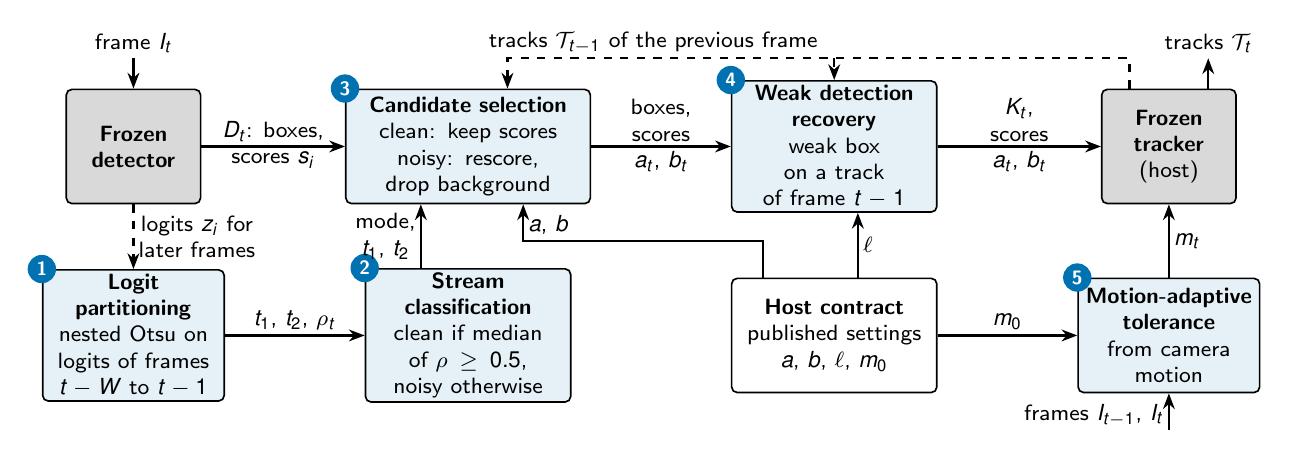
\begin{tikzpicture}[x=1cm, y=1cm, font=\footnotesize,
  blk/.style={draw, line width=0.6pt, rounded corners=2pt, align=center, minimum height=14.5mm, inner sep=1.5pt},
  frozen/.style={blk, fill=oklight, text width=16mm},
  proc/.style={blk, fill=okblue!10, text width=25mm},
  procs/.style={blk, fill=okblue!10, text width=22mm},
  cont/.style={blk, fill=white, text width=25mm},
  num/.style={circle, fill=okblue, text=white, font=\scriptsize\bfseries, inner sep=0.8pt, minimum size=3.6mm},
  arr/.style={-{Stealth[length=2mm]}, line width=0.8pt},
  past/.style={arr, dashed},
  lab/.style={font=\footnotesize, align=center, inner sep=1.5pt}]
% column centres (row A: detector, candidate choice, rescue, tracker; row B: below them)
\def\ca{0.95}\def\cb{5.2}\def\cc{9.85}\def\cd{14.1}
\def\ra{0}\def\rb{-2.4}
% ---------------- blocks
\node[frozen] (det)  at (\ca,\ra) {\textbf{Frozen}\\\textbf{detector}};
\node[proc, text width=30mm] (cand) at (\cb,\ra) {\textbf{Candidate selection}\\clean: keep scores\\noisy: rescore,\\drop background};
\node[proc]   (res)  at (\cc,\ra) {\textbf{Weak detection}\\\textbf{recovery}\\weak box on a track\\of frame $t-1$};
\node[frozen] (trk)  at (\cd,\ra) {\textbf{Frozen}\\\textbf{tracker}\\(host)};
\node[procs]  (stat) at (\ca,\rb) {\textbf{Logit}\\\textbf{partitioning}\\nested Otsu on\\logits of frames\\$t-W$ to $t-1$};
\node[proc]   (mode) at (\cb,\rb) {\textbf{Stream}\\\textbf{classification}\\clean if median\\of $\rho\ge0.5$,\\noisy otherwise};
\node[cont]   (hc)   at (\cc,\rb) {\textbf{Host contract}\\published settings\\$a$, $b$, $\ell$, $m_0$};
\node[procs]  (tol)  at (\cd,\rb) {\textbf{Motion-adaptive}\\\textbf{tolerance}\\from camera\\motion};
% step numbers
\foreach \n/\b in {1/stat, 2/mode, 3/cand, 4/res, 5/tol}
  \node[num] at (\b.north west) {\n};
% ---------------- data of frame t
\draw[arr] (\ca,1.12) node[lab, above] {frame $I_t$} -- (det.north);
\draw[arr] (det.east) -- node[lab, above] {$D_t$: boxes,} node[lab, below] {scores $s_i$} (cand.west);
\draw[arr] (cand.east) -- node[lab, above] {boxes,\\scores} node[lab, below] {$a_t$, $b_t$} (res.west);
\draw[arr] (res.east) -- node[lab, above] {$K_t$,\\scores} node[lab, below] {$a_t$, $b_t$} (trk.west);
\draw[arr] ([xshift=5mm]trk.north) -- ([xshift=5mm]trk.north |- 0,1.12) node[lab, above] {tracks $\mathcal{T}_t$};
\draw[arr] (stat.east) -- node[lab, above] {$t_1$, $t_2$, $\rho_t$} (mode.west);
\draw[arr] ([xshift=-6mm]mode.north) -- node[lab, left] {mode,\\$t_1$, $t_2$} ([xshift=-6mm]cand.south);
\draw[arr] ([xshift=-9mm]hc.north) |- ([xshift=7mm]cand.south |- 0,-1.2) -- node[lab, pos=0.45, right] {$a$, $b$} ([xshift=7mm]cand.south);
\draw[arr] ([xshift=3mm]hc.north) -- node[lab, right] {$\ell$} ([xshift=3mm]res.south);
\draw[arr] (hc.east) -- node[lab, above] {$m_0$} (tol.west);
\draw[arr] (\cd,-3.6) -- node[lab, left, pos=0.4] {frames $I_{t-1}$, $I_t$} (tol.south);
\draw[arr] (tol.north) -- node[lab, right] {$m_t$} (trk.south);
% ---------------- data kept from earlier frames
\draw[past] (det.south) -- node[lab, right] {logits $z_i$ for\\later frames} (stat.north);
\draw[past] ([xshift=-5mm]trk.north) -- ([xshift=-5mm]trk.north |- 0,1.12) -| ([xshift=5mm]cand.north);
\draw[past] (\cc,1.12) -- (res.north);
\node[lab, above] at (7.55,1.12) {tracks $\mathcal{T}_{t-1}$ of the previous frame};
\end{tikzpicture}
\end{document}
